\documentclass[fleqn, 11pt,letterpaper]{article}
\usepackage[letterpaper,left=2.5cm, right=2.5cm, top=2.5cm, bottom=2.5cm]{geometry}
\usepackage{graphicx} % Required for inserting images
\usepackage{booktabs} % For \toprule, \midrule, \bottomrule
\usepackage{float}    % For [H] float placement
\usepackage{svg}      % For \includesvg command
\svgsetup{inkscapelatex=false}
\usepackage{makecell} % For \makecell in table headers
\usepackage{amsmath, amssymb}
\usepackage{array} % para columnas p{} dentro de array
\usepackage{tabularx}
\usepackage{xcolor}
\usepackage{tikz}  % Diagrama de la red actual
\usetikzlibrary{arrows.meta, positioning, calc}
% Colores de los centros de distribución (los mismos de las figuras de resultados)
\definecolor{cediCali}{HTML}{2A78D6}
\definecolor{cediPereira}{HTML}{EB6834}
\definecolor{cediBogota}{HTML}{1BAF7A}
\definecolor{cediMedellin}{HTML}{EDA100}
\definecolor{cediBarranquilla}{HTML}{E87BA4}
\usepackage[nottoc,numbib]{tocbibind} % numera la sección de referencias

\title{Rediseño de la Red de Distribución en una Empresa de Manufactura de Artículos para el Hogar}
\author{
    Mateo Vásquez Jaramillo\\Maestría en ingeniería\\Universidad EAFIT\\
    \texttt{mvasquezj@eafit.edu.co}
    }
\date{}

\begin{document}
\maketitle

\section{Introducción}
\textcolor{blue}{En un entorno de mercado cada vez más competitivo, la ubicación estratégica de los centros de distribución y el diseño de la red de distribución en función de los puntos de demanda se han consolidado como factores clave para reducir los costos logísticos y sostener el nivel de servicio al cliente. Las decisiones sobre cuántos centros operar, dónde ubicarlos y con qué capacidad tienen efectos de largo plazo sobre la estructura de costos de una organización, por lo que su análisis mediante modelos de optimización resulta especialmente relevante.}

\vspace{1mm}

\textcolor{blue}{En este contexto, el presente caso de estudio analiza el rediseño de la red de distribución de una empresa colombiana del sector manufacturero de artículos para el hogar, con más de 70 años en el mercado. El ejercicio surge de una solicitud expresa del equipo directivo, interesado en identificar el mejor diseño posible dadas las variables y condiciones de la operación. El principal reto consiste en satisfacer la totalidad de la demanda cumpliendo con el nivel de servicio del 97\,\% declarado por la compañía, el cual se destaca como una ventaja competitiva dentro de este sector económico.}

\vspace{1mm}

\textcolor{blue}{La red de distribución actual opera en dos escalones: una planta de producción central despacha el producto terminado hacia cinco centros de distribución ubicados en Bogotá, Medellín, Barranquilla, Cali y Pereira, y desde estos se atiende la demanda de los 32 departamentos del país, cada uno asignado a un único centro. Durante el año 2025 la red movilizó 139.623 unidades, equivalentes a 22.911\,m$^3$ y a 16.606 posiciones de estiba, con una demanda altamente concentrada: Antioquia, Bogotá D.C. y Valle del Cauca representan cerca del 50\,\% del total.}

\vspace{1mm}

\textcolor{blue}{Para abordar este problema se propone un modelo de programación lineal entera mixta que mantiene fija la ubicación de la planta, dado que su traslado implicaría costos fijos significativamente superiores a los de la operación actual. El modelo determina de forma simultánea qué centros de distribución habilitar, de qué tamaño (desde XS hasta XL, según las posiciones de estiba movilizadas por día) y cómo asignar los flujos de cada categoría de producto hacia las zonas de demanda, minimizando el costo logístico anual compuesto por el transporte en ambas fases, los costos fijos de operación de los centros y los costos variables de manejo de materiales.}

\vspace{1mm}

\textcolor{blue}{Es importante precisar que los datos presentados en este trabajo han sido normalizados y homologados. Por lo tanto, no representan la realidad operativa de la organización, sino una representación funcional de su red de distribución y de sus puntos de demanda. Así mismo, las categorías y artículos utilizados no corresponden a los nombres de los artículos comercializados o manufacturados por la compañía.}

\vspace{1mm}

\textcolor{blue}{El documento se organiza de la siguiente manera: la Sección 2 presenta la revisión de literatura; la Sección 3 describe el caso de estudio y el diseño actual de la red; la Sección 4 formula el modelo matemático; la Sección 5 reporta los experimentos computacionales, y la Sección 6 presenta las conclusiones.}

\section{Revisión de Literatura}
El diseño de redes de distribución es un problema clásico de la investigación de operaciones aplicada a la logística: consiste en determinar el número, la ubicación y la capacidad de las instalaciones, junto con los flujos de producto entre ellas, de manera que la demanda se atienda al menor costo posible. Las revisiones de Aikens \cite{Aik85}, Klose y Drexl \cite{Klo05} y Melo et al. \cite{Mel09} organizan esta literatura a partir de los modelos de localización de instalaciones y de su papel en la gestión de la cadena de suministro. De manera complementaria, ReVelle y Laporte \cite{Rev96} discuten variantes del problema de localización de plantas con múltiples productos, y Ortiz-Astorquiza et al. \cite{Ort17} revisan los problemas de localización con varios niveles de instalaciones.

Una primera línea de trabajo se concentra en redes con múltiples productos en las que la capacidad de cada instalación es un dato del problema. El trabajo de Geoffrion y Graves \cite{Geo74} es la referencia fundacional: formula el diseño de un sistema de distribución multiproducto con plantas, centros de distribución y zonas de clientes, y lo resuelve mediante descomposición de Benders. Hindi y Basta \cite{Hin94} y Hindi et al. \cite{Hin98} abordan problemas de distribución y localización de dos etapas con múltiples productos; en el segundo de estos trabajos, cada centro de distribución candidato tiene un costo fijo de apertura, un costo de operación y una capacidad máxima. Pirkul y Jayaraman \cite{Pir96, Pir98} proponen modelos de programación entera mixta para localizar plantas y bodegas en sistemas con múltiples productos, con el objetivo de minimizar los costos de transporte y distribución y los costos fijos de apertura y operación de las instalaciones. Hinojosa et al. \cite{Hin00} extienden el problema de dos escalones con múltiples productos a un horizonte de varios periodos.

Una segunda línea incorpora la capacidad de las instalaciones como una decisión que se toma sobre un conjunto discreto de alternativas. Shulman \cite{Shu91} estudia un problema dinámico de localización de plantas en el que las expansiones solo pueden hacerse en tamaños discretos, y Lee \cite{Lee96} formula una red de distribución de dos etapas en la que cada centro de distribución debe pertenecer a uno de varios tipos estandarizados. Mazzola y Neebe \cite{Maz99} consideran un problema de localización capacitado con múltiples familias de productos, en el que cada sitio elige entre tipos de instalación con capacidades y costos fijos diferentes. Correia y Captivo \cite{Cor03b} tratan el caso en el que la capacidad se instala por módulos, y Amiri \cite{Ami05} permite varios niveles de capacidad para plantas y bodegas en el diseño de una red de distribución. Más recientemente, Li et al. \cite{Li14} incorporan costos de manipulación en un problema de localización capacitado de dos etapas, y Wu et al. \cite{Wu15b, Wu19} agregan la selección del tamaño de los depósitos; en \cite{Wu19}, la función objetivo suma los costos de apertura, de manipulación, de transporte y de asignación. Irawan y Jones \cite{Ira19} estudian el caso con múltiples productos en una cadena de dos etapas, donde cada depósito candidato dispone de varios niveles de capacidad y se minimizan los costos fijos de apertura y los costos de transporte. Ashtab et al. \cite{Ash19} relajan la condición de elegir un único nivel y permiten que una instalación combine varios niveles de capacidad.

En cuanto a las aplicaciones, existe una tradición amplia de estudios de rediseño de redes apoyados en modelos de optimización. Camm et al. \cite{Cam97} combinan programación entera, modelos de optimización de redes y un sistema de información geográfica para reestructurar la cadena de suministro de Procter \& Gamble en Norteamérica, con una reducción cercana al 20\,\% en el número de plantas. Sery et al. \cite{Ser01} usan modelos basados en programación lineal para evaluar el compromiso entre costo y servicio en la red de BASF, donde las entregas al día siguiente pasaron del 77\,\% al 90\,\%. Robinson et al. \cite{Rob93} desarrollan un sistema de apoyo a la decisión para diseñar sistemas de distribución de dos escalones con múltiples productos en DowBrands. Otros casos documentados incluyen empresas de alimentos y bebidas \cite{Poo94, Kok95, Wou02}, una compañía farmacéutica \cite{Rab08} y, más recientemente, McDonald's China \cite{Tan25}. En el contexto latinoamericano, Guazzelli y da Cunha \cite{Gua14} proponen un modelo de programación entera mixta para localizar los centros de distribución de una empresa de alimentos, que considera múltiples productos, costos fijos y variables de las instalaciones y economías de escala asociadas con el tamaño de los centros, y reportan ahorros de hasta 8,3\,\% en los costos de operación.

El modelo que se propone en este trabajo pertenece a la segunda línea. Como la red estudiada tiene una única planta, sin decisiones de apertura ni restricciones de capacidad, la primera etapa de transporte solo agrega un costo unitario al flujo que pasa por cada centro de distribución. En consecuencia, su estructura es cercana a la del problema de localización capacitado con múltiples productos y elección del tipo de instalación de Mazzola y Neebe \cite{Maz99}, y a la del modelo con niveles de capacidad de Irawan y Jones \cite{Ira19}. A diferencia de este último, incluye un costo variable de manejo de materiales en los centros de distribución, un componente que también aparece en \cite{Li14, Wu19}. El aporte de este trabajo no radica entonces en una formulación nueva, sino en la adaptación de formulaciones establecidas al rediseño de la red de distribución de una empresa de manufactura de artículos para el hogar.

\section{Caso de Estudio}
\subsection{Planteamiento del caso de estudio}
Una empresa del sector manufacturero con más de 70 años en el mercado de productos domésticos desea evaluar la viabilidad tanto operativa como financiera de reubicar sus Centros de distribución; es de aclarar que únicamente se plantea el desarrollo del ejercicio con la reubicación de los centros de distribución de cada una de las zonas de demanda agregada debido a que para efectos prácticos, se considera que el traslado de la planta de producción implicaría costos fijos significativamente elevados frente a los costos de operación actuales, los cuales ya han sido depreciados contablemente a lo largo del tiempo.

\subsection{Descripción del proceso de distribución}
La compañía fabrica y comercializa artículos para el hogar, principalmente electrodomésticos de línea blanca y pequeños electrodomésticos, organizados en 20 categorías de producto y 160 referencias (SKU). Toda la producción se concentra en una única planta ubicada en Cali, desde la cual se abastece la red de distribución nacional. El proceso de distribución se desarrolla en dos escalones: el transporte primario, que lleva el producto terminado de la planta a los centros de distribución, y la distribución secundaria, que lo lleva de los centros de distribución a los clientes.

En el primer escalón, el producto terminado sale de la planta hacia cinco centros de distribución. El centro de distribución de Cali se encuentra acoplado a la planta, por lo que recibe la producción mediante un traslado corto en camión sencillo. Los centros de distribución de Bogotá, Medellín, Barranquilla y Pereira se abastecen por carretera con una flota de cuatro tipos de vehículo: camioneta o furgón, camión sencillo, doble troque y tractocamión. Como los productos no son apilables, cada vehículo transporta una cantidad de estibas limitada por las posiciones disponibles en su plataforma y no por su capacidad en peso.

En cada centro de distribución se realizan las operaciones de recepción y descargue, almacenamiento en posiciones de estiba, alistamiento de pedidos y despacho. Para ello, cada centro cuenta con personal de dirección, coordinación, control de inventarios, montacarguistas y operarios de bodega, así como con montacargas y un sistema de gestión de bodegas. Los centros mantienen un inventario de seguridad dimensionado para cumplir el nivel de servicio del 97\,\% definido por la compañía, considerando la variabilidad de la demanda diaria y el tiempo de reposición desde la planta.

En el segundo escalón, cada centro de distribución atiende los pedidos de los clientes ubicados en su zona de influencia. Cada municipio es atendido por un único centro de distribución, de acuerdo con una asignación geográfica fija. Durante 2025 la compañía atendió 2.370 pedidos, con 3.838 líneas de pedido, de 188 clientes ubicados en 79 municipios de 31 departamentos. Los clientes pertenecen a tres canales comerciales: minorista (38,7\,\% de las líneas de pedido), mayorista (31,0\,\%) y comercio electrónico (30,4\,\%). Los despachos hacia los clientes se realizan con la misma flota de cuatro tipos de vehículo, eligiendo en cada ruta la combinación de vehículos que permite movilizar el volumen requerido al menor costo.

La unidad con la que se mide el flujo en todo el proceso es la posición de estiba (Sección~\ref{sec:unidad_flujo}). En 2025 la red movilizó 1.176.918 posiciones de estiba hacia los clientes.

\subsection{Datos del caso de estudio}

\subsubsection{Unidad de medida del flujo logístico}
\label{sec:unidad_flujo}

La unidad de medida con la que se definen el flujo y la capacidad de la red es la posición de estiba, entendida como el espacio que ocupa una estiba cargada, ya sea en la plataforma de un vehículo o en la bodega de un centro de distribución.

Los productos de la compañía son heterogéneos en peso y volumen: una nevera ocupa casi dos metros cúbicos, mientras que un pequeño electrodoméstico ocupa una fracción de ese espacio. Por esta razón, ni las unidades vendidas ni el peso ni el volumen permiten medir de forma homogénea el uso de los recursos logísticos. La posición de estiba sí lo permite, porque refleja el espacio que efectivamente ocupa el producto. Además, como la carga no es apilable, el número de estibas que transporta un vehículo está limitado por las posiciones de su plataforma y no por su capacidad en peso, de modo que la misma unidad sirve para medir el almacenamiento y el transporte.

La demanda en posiciones de estiba se calcula para cada línea de pedido como
\begin{equation*}
    \text{posiciones de estiba} \; = \; \left\lceil \frac{\text{unidades pedidas}}{\text{unidades por estiba del SKU}} \right\rceil ,
\end{equation*}
donde las unidades por estiba de cada SKU se determinan a partir de su peso, su volumen y su factor de empaque. El redondeo hacia arriba supone que cada línea de pedido se despacha en estibas completas de una sola referencia, sin consolidar referencias distintas en una misma estiba, lo que corresponde a una medición conservadora del espacio requerido.

Esta unidad se usa de manera consistente en todo el modelo: la demanda $d_{ik}$, la capacidad de los centros de distribución $a_s$ (posiciones de estiba movilizadas por día, Tabla~\ref{tab:tamano_cedi}), la capacidad de los vehículos $q_t$ y los costos unitarios $h_{js}$ y $\varphi$ se expresan en posiciones de estiba. Cuando un costo está definido en otra unidad, como el costo de manejo por tonelada recibida, se convierte con la relación promedio de 0,11 toneladas por posición de estiba observada en 2025.

\subsubsection{Datos de demanda agregada y definición de zonas de demanda}
La demanda actual se encuentra segregada en 32 departamentos, donde cada uno de ellos es atendido por uno de los 5 centros de distribución que actualmente tiene la empresa.

A continuación, en la Tabla~\ref{tab:demanda_departamentos} se presenta el volumen de unidades movilizadas en cada una de las zonas para el periodo 2025; asimismo, en la Tabla~\ref{tab:demanda_nodos} se presenta el volumen de unidades movilizadas por cada uno de los centros de distribución.

\raggedbottom
% -------------------------------------------
% Tabla: Demanda agregada por departamentos
% -------------------------------------------
\begin{table}[H]
\centering
\caption{Demanda agregada por departamentos, 2025 (unidades)}
\label{tab:demanda_departamentos}
\small
\renewcommand{\arraystretch}{1.1}
\begin{tabular}{lrrr}
\toprule
\textbf{Departamento} & \textbf{Cantidades} & \textbf{\% Participación} & \textbf{\% Part. acumulado} \\
\midrule
Antioquia          & 906.641 & 22,50\% & 22,5\%  \\
Cundinamarca       & 861.888 & 21,39\% & 43,9\%  \\
Valle del Cauca    & 512.484 & 12,72\% & 56,6\%  \\
Atlántico          & 232.035 &  5,76\% & 62,4\%  \\
Casanare           & 130.112 &  3,23\% & 65,6\%  \\
La Guajira         & 126.002 &  3,13\% & 68,7\%  \\
Boyacá             & 110.175 &  2,73\% & 71,5\%  \\
Norte de Santander &  91.883 &  2,28\% & 73,7\%  \\
Arauca             &  84.296 &  2,09\% & 75,8\%  \\
Cesar              &  84.015 &  2,09\% & 77,9\%  \\
Tolima             &  77.410 &  1,92\% & 79,8\%  \\
Sucre              &  68.306 &  1,70\% & 81,5\%  \\
Córdoba            &  66.216 &  1,64\% & 83,2\%  \\
Huila              &  65.757 &  1,63\% & 84,8\%  \\
Magdalena          &  60.448 &  1,50\% & 86,3\%  \\
Cauca              &  58.959 &  1,46\% & 87,8\%  \\
Caldas             &  56.222 &  1,40\% & 89,2\%  \\
Vaupés             &  54.876 &  1,36\% & 90,5\%  \\
Caquetá            &  47.959 &  1,19\% & 91,7\%  \\
Guaviare           &  46.663 &  1,16\% & 92,9\%  \\
Risaralda          &  45.052 &  1,12\% & 94,0\%  \\
Santander          &  42.888 &  1,06\% & 95,1\%  \\
Meta               &  38.100 &  0,95\% & 96,0\%  \\
Chocó              &  35.843 &  0,89\% & 96,9\%  \\
Putumayo           &  33.679 &  0,84\% & 97,7\%  \\
Quindío            &  31.260 &  0,78\% & 98,5\%  \\
Bolívar            &  23.142 &  0,57\% & 99,1\%  \\
Amazonas           &  17.038 &  0,42\% & 99,5\%  \\
Nariño             &  10.938 &  0,27\% & 99,8\%  \\
Guainía            &   4.578 &  0,11\% & 99,9\%  \\
Vichada            &   4.395 &  0,11\% & 100,0\% \\
\midrule
\textbf{Total general} & \textbf{4.029.260} & \textbf{100,00\%} & \\
\bottomrule
\end{tabular}
\end{table}
Luego de entender el comportamiento de la demanda agregada para el año 2025, se analiza las cantidades de posiciones de estiba movilizadas por cada uno de los centros de distribución actualmente ubicados, con el fin de determinar el costo de la operación en cada centro logístico en función de las Posiciones de estiba movilizadas.


% -------------------------------------------
% Tabla 2: Demanda, volumen y posiciones de estiba por Centro Logístico
% -------------------------------------------
\begin{table}[H]
\centering
\caption{Demanda, volumen movilizado y posiciones de estiba por Centro Logístico}
\label{tab:demanda_nodos}
\begin{tabular}{lrrr}
\toprule
\textbf{Centro Logístico} & \textbf{Cantidades} & \textbf{MT3 Movilizados} & \textbf{Posiciones Estiba} \\
\midrule
CEDI-BOG      & 50.382  & 8.838  & 6.446  \\
CEDI-MED      & 35.771  & 5.355  & 3.909  \\
CEDI-BAQ      & 20.861  & 3.546  & 2.515  \\
PLT-CALI      & 20.440  & 3.575  & 2.603  \\
CEDI-PER      & 12.169  & 1.597  & 1.134  \\
\midrule
\textbf{Total general} & \textbf{139.623} & \textbf{22.911} & \textbf{16.606} \\
\bottomrule
\end{tabular}
\end{table}

% -------------------------------------------
% Tabla 3: Posiciones por día por CEDI
% -------------------------------------------
\begin{table}[H]
\centering
\caption{Posiciones por día por CEDI, año 2025}
\label{tab:posiciones_mensuales}
\small
\setlength{\tabcolsep}{4pt}
\renewcommand{\arraystretch}{1.2}
\resizebox{\linewidth}{!}{%
\begin{tabular}{l *{12}{c} c}
\toprule
\textbf{CEDI} & ene & feb & mar & abr & may & jun & jul & ago & sept & oct & nov & dic & \makecell{Total\\general} \\
\midrule
CEDI-PER  &  2 &  6 &  5 &  3 &  4 &  4 &  2 &  4 &  2 &  3 &  7 &  3 &  45 \\
CEDI-MED  & 12 & 14 & 12 &  9 &  9 & 10 &  6 & 10 & 10 &  8 & 18 & 17 & 135 \\
CEDI-CALI &  7 &  5 &  8 &  6 &  8 &  9 &  8 &  8 &  7 &  9 &  6 & 12 &  93 \\
CEDI-BOG  & 23 & 22 & 15 & 15 & 23 & 17 & 13 & 13 & 16 & 15 & 20 & 28 & 220 \\
CEDI-BAQ  &  8 &  5 &  4 &  8 &  9 &  6 &  9 &  5 & 10 &  7 &  8 & 12 &  91 \\
\midrule
\textbf{Total general} & \textbf{52} & \textbf{52} & \textbf{44} & \textbf{41} & \textbf{53} & \textbf{46} & \textbf{38} & \textbf{40} & \textbf{45} & \textbf{42} & \textbf{59} & \textbf{72} & \textbf{584} \\
\bottomrule
\end{tabular}%
}
\end{table}

% -------------------------------------------
% Tabla 4: Estadísticos y stock de seguridad
% -------------------------------------------
\begin{table}[H]
\centering
\caption{Estadísticos de demanda y cálculo del stock de seguridad por CEDI}
\label{tab:stock_seguridad}
\small
\setlength{\tabcolsep}{4pt}
\renewcommand{\arraystretch}{1.25}
\resizebox{\linewidth}{!}{%
\begin{tabular}{l *{11}{c}}
\toprule
 & \multicolumn{4}{c}{\textbf{Estadísticos}} & \multicolumn{7}{c}{\textbf{Parámetros de inventario}} \\
\cmidrule(lr){2-5} \cmidrule(lr){6-12}
\textbf{CEDI} & Mín & Máx & Prom. & Desv. &
\makecell{Nivel de\\servicio} & \makecell{Peso\\demanda} & \makecell{Lead time\\(días)} &
\makecell{Demanda en\\1 lead time} & $Z^{*}$ & SS & Posiciones \\
\midrule
CEDI-PER  &  2 &  7 &  4 & 1,61 & 97\% &   8\% & 1   &  4 & 1,88 &  4 &   8 \\
CEDI-MED  &  6 & 18 & 11 & 3,58 & 97\% &  23\% & 2   & 23 & 1,88 & 14 &  37 \\
CEDI-CALI &  5 & 12 &  8 & 1,82 & 97\% &  16\% & 0,5 &  4 & 1,88 &  2 &   6 \\
CEDI-BOG  & 13 & 28 & 18 & 4,78 & 97\% &  38\% & 2   & 37 & 1,88 & 18 &  55 \\
CEDI-BAQ  &  4 & 12 &  8 & 2,32 & 97\% &  16\% & 4   & 31 & 1,88 & 18 &  49 \\
\midrule
\textbf{Total general} & \textbf{38} & \textbf{72} & \textbf{49} & \textbf{9,67} & \textbf{97\%} & \textbf{100\%} & \textbf{2,0} & \textbf{20} & \textbf{1,88} & \textbf{26} & \textbf{155} \\
\bottomrule
\end{tabular}%
}
\end{table}

\subsubsection{Definición tamaños y capacidades centros de distribución}

Para la definición de los tamaños y capacidades requeridas se toma como referencia una definición de regla de negocio de garantizar un nivel de servicio del 97\%. En la Tabla~\ref{tab:posiciones_nivel_servicio} se presenta cuales son las posiciones de estiba requeridos diariamente para garantizar la operación a determinado nivel de servicio.

%-----------------------------
% Tabla 5: Posiciones de estiba por nivel de servicio
% -----------------------------
\begin{table}[H]
\centering
\caption{Posiciones de estiba por nivel de servicio y CEDI}

\label{tab:posiciones_nivel_servicio}
\renewcommand{\arraystretch}{1.2}
\begin{tabular}{l *{6}{r}}
\toprule
 & \multicolumn{6}{c}{\textbf{Nivel de servicio}} \\
\cmidrule(lr){2-7}
\textbf{CEDI} & 85\% & 90\% & 95\% & \textbf{97\%} & 98\% & 99\% \\
\midrule
CEDI-PER  &  6 &  7 &  7 & \textbf{8}  &  8 &  8 \\
CEDI-MED  & 31 & 33 & 35 & \textbf{37} & 38 & 40 \\
CEDI-CALI &  5 &  6 &  6 & \textbf{6}  &  6 &  7 \\
CEDI-BOG  & 47 & 50 & 53 & \textbf{55} & 57 & 60 \\
CEDI-BAQ  & 41 & 43 & 47 & \textbf{49} & 51 & 53 \\
\midrule
Total & 130 & 139 & 148 & \textbf{155} & 160 & 168 \\
\bottomrule
\end{tabular}
\end{table}

De acuerdo con la cantidad de posiciones día movilizadas por cada uno de los centros de distribución para cada uno de los niveles de servicio planteados, se determinan los siguientes parámetros en la Tabla~\ref{tab:tamano_cedi}  para determinar los tamaños de los centros de distribución:

% -----------------------
% Tabla 6: Clasificación del tamaño de CEDI
% -----------------------
\begin{table}[H]
\centering
\caption{Tamaño de CEDI según posiciones de estiba movilizadas por día}
\label{tab:tamano_cedi}
\renewcommand{\arraystretch}{1.2}
\begin{tabular}{ccc}
\toprule
 & \multicolumn{2}{c}{\textbf{Posiciones de estiba por día}} \\
\cmidrule(lr){2-3}
\textbf{Tamaño} & \textbf{Mínimo} & \textbf{Máximo} \\
\midrule
XS & 1    & 360  \\
S  & 361  & 720  \\
M  & 721  & 1.080 \\
L  & 1.081 & 1.440 \\
XL & 1.441 & 1.800 \\
\bottomrule
\end{tabular}
\end{table}

En consecuencia, se determinan los siguientes tamaños para cada centro de distribución
% ============================================================
% Tabla 7: Tamaño de CEDI por nivel de servicio
% ============================================================
\begin{table}[H]
\centering
\caption{Tamaño de CEDI por nivel de servicio}
\label{tab:tamano_nivel_servicio}
\renewcommand{\arraystretch}{1.2}
\begin{tabular}{l *{6}{c}}
\toprule
 & \multicolumn{6}{c}{\textbf{Nivel de servicio}} \\
\cmidrule(lr){2-7}
\textbf{CEDI} & 85\% & 90\% & 95\% & \textbf{97\%} & 98\% & 99\% \\
\midrule
CEDI-PER  & XS & XS & XS & \textbf{XS} & XS & XS \\
CEDI-MED  & M  & M  & M  & \textbf{L}  & L  & L  \\
CEDI-CALI & XS & XS & XS & \textbf{XS} & XS & XS \\
CEDI-BOG  & L  & XL & XL & \textbf{XL} & XL & XL \\
CEDI-BAQ  & L  & L  & L  & \textbf{XL} & XL & XL \\
\bottomrule
\end{tabular}
\end{table}
\subsubsection{Demanda proyectada próximos años}

\subsection{Diseño actual}
La red de distribución actual está conformada por la planta de Cali, cinco centros de distribución y las 79 zonas de demanda asignadas a ellos, como se muestra en la Figura~\ref{fig:red_actual}. Bogotá es el centro de distribución de mayor volumen: atiende 27 municipios de 14 departamentos del centro, el oriente y el sur del país, y concentra el 41,2\,\% del flujo. Le siguen Medellín, que atiende Antioquia y Chocó con el 22,4\,\% del flujo; Barranquilla, que atiende siete departamentos de la Costa Caribe con el 16,8\,\%; Cali, que atiende el suroccidente con el 16,7\,\%, y Pereira, que atiende el Eje Cafetero con el 2,9\,\%. El tamaño de cada centro corresponde a las posiciones de estiba movilizadas por día para el nivel de servicio del 97\,\% (Tabla~\ref{tab:tamano_nivel_servicio}), salvo el centro de distribución de Cali, que por estar acoplado a la planta opera con tamaño XL.

\begin{figure}[H]
\centering
\resizebox{\linewidth}{!}{%
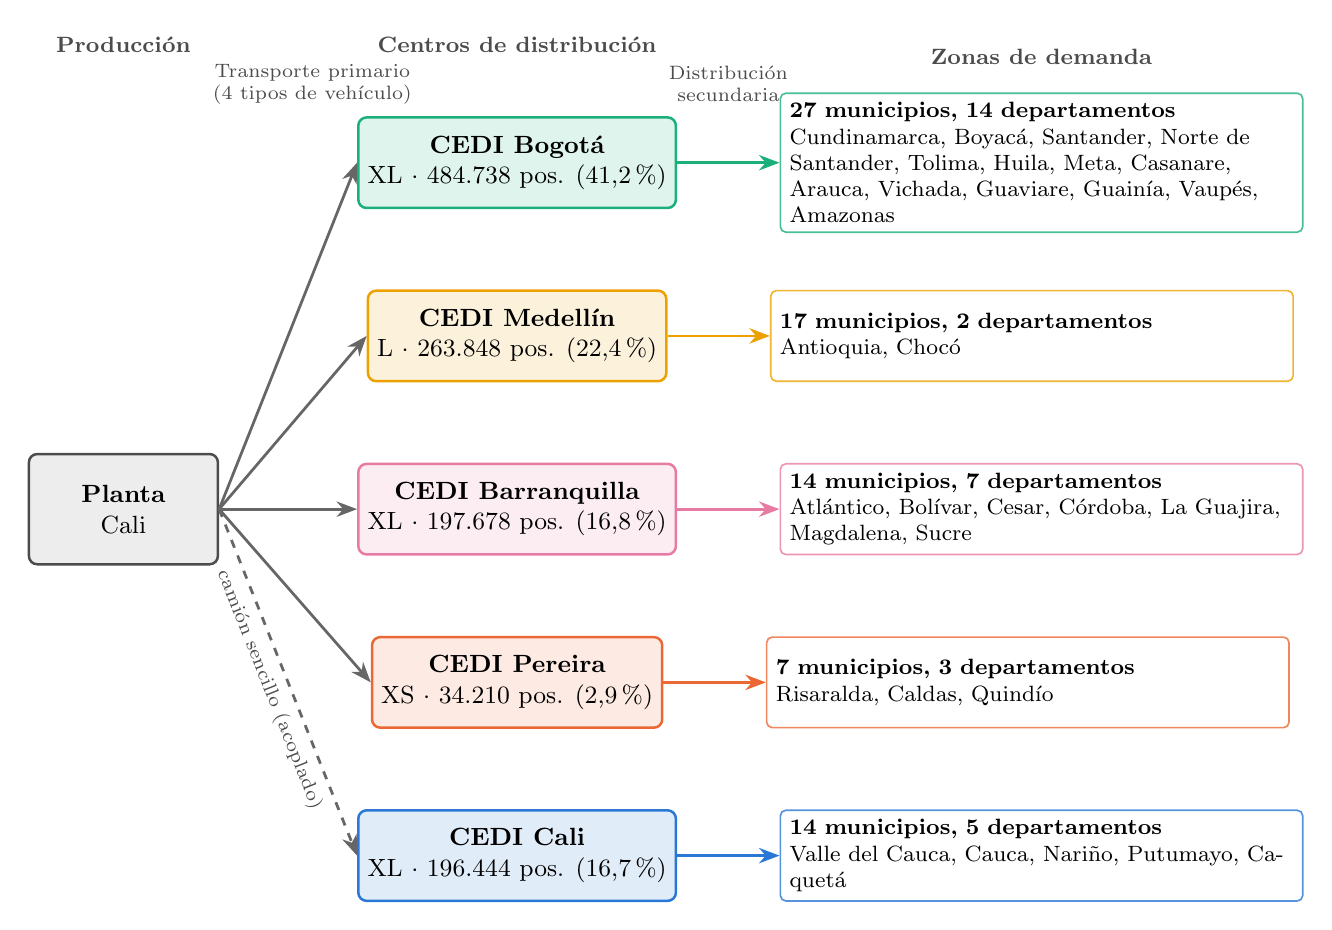
\begin{tikzpicture}[
    font=\small,
    planta/.style={draw=black!70, fill=black!7, rounded corners=3pt, minimum width=2.4cm,
                   minimum height=1.4cm, align=center, line width=0.9pt},
    cedi/.style={draw=#1, fill=#1!14, rounded corners=3pt, minimum width=3.6cm, minimum height=1.15cm,
                 align=center, line width=0.9pt},
    zona/.style={draw=#1!80, fill=white, rounded corners=2pt, text width=6.4cm, minimum height=1.15cm,
                 align=left, font=\footnotesize, line width=0.6pt},
    primario/.style={-{Stealth[length=2.6mm]}, line width=1pt, draw=black!60},
    secundario/.style={-{Stealth[length=2.6mm]}, line width=1pt, draw=#1},
]
% Planta
\node[planta] (P) at (0,0) {\textbf{Planta}\\Cali};

% Centros de distribución (tamaño actual y flujo anual en posiciones de estiba)
\node[cedi=cediBogota]       (BOG) at (5.0, 4.4)  {\textbf{CEDI Bogotá}\\XL $\cdot$ 484.738 pos. (41,2\,\%)};
\node[cedi=cediMedellin]     (MED) at (5.0, 2.2)  {\textbf{CEDI Medellín}\\L $\cdot$ 263.848 pos. (22,4\,\%)};
\node[cedi=cediBarranquilla] (BAQ) at (5.0, 0.0)  {\textbf{CEDI Barranquilla}\\XL $\cdot$ 197.678 pos. (16,8\,\%)};
\node[cedi=cediPereira]      (PER) at (5.0, -2.2) {\textbf{CEDI Pereira}\\XS $\cdot$ 34.210 pos. (2,9\,\%)};
\node[cedi=cediCali]         (CAL) at (5.0, -4.4) {\textbf{CEDI Cali}\\XL $\cdot$ 196.444 pos. (16,7\,\%)};

% Zonas de demanda atendidas por cada centro de distribución
\node[zona=cediBogota, right=1.3cm of BOG] (ZBOG) {\textbf{27 municipios, 14 departamentos}\\Cundinamarca, Boyacá, Santander, Norte de Santander, Tolima, Huila, Meta, Casanare, Arauca, Vichada, Guaviare, Guainía, Vaupés, Amazonas};
\node[zona=cediMedellin, right=1.3cm of MED] (ZMED) {\textbf{17 municipios, 2 departamentos}\\Antioquia, Chocó};
\node[zona=cediBarranquilla, right=1.3cm of BAQ] (ZBAQ) {\textbf{14 municipios, 7 departamentos}\\Atlántico, Bolívar, Cesar, Córdoba, La Guajira, Magdalena, Sucre};
\node[zona=cediPereira, right=1.3cm of PER] (ZPER) {\textbf{7 municipios, 3 departamentos}\\Risaralda, Caldas, Quindío};
\node[zona=cediCali, right=1.3cm of CAL] (ZCAL) {\textbf{14 municipios, 5 departamentos}\\Valle del Cauca, Cauca, Nariño, Putumayo, Caquetá};

% Transporte primario: planta -> centros de distribución
\foreach \cedi in {BOG, MED, BAQ, PER} {
    \draw[primario] (P.east) -- (\cedi.west);
}
\draw[primario, dashed] (P.east) -- node[below, sloped, font=\scriptsize, text=black!70] {camión sencillo (acoplado)} (CAL.west);

% Distribución secundaria: centros de distribución -> zonas de demanda
\draw[secundario=cediBogota]       (BOG.east) -- (ZBOG.west);
\draw[secundario=cediMedellin]     (MED.east) -- (ZMED.west);
\draw[secundario=cediBarranquilla] (BAQ.east) -- (ZBAQ.west);
\draw[secundario=cediPereira]      (PER.east) -- (ZPER.west);
\draw[secundario=cediCali]         (CAL.east) -- (ZCAL.west);

% Encabezados de los escalones
\node[font=\footnotesize\bfseries, text=black!70] at (0, 5.9)   {Producción};
\node[font=\footnotesize\bfseries, text=black!70] at (5.0, 5.9) {Centros de distribución};
\node[font=\footnotesize\bfseries, text=black!70] at ($(ZBOG.north)+(0,0.45)$) {Zonas de demanda};
\node[font=\scriptsize, text=black!70, align=center] at (2.4, 5.4) {Transporte primario\\(4 tipos de vehículo)};
\node[font=\scriptsize, text=black!70, align=center] at ($(BOG.east)!0.5!(ZBOG.west)+(0,1.0)$) {Distribución\\secundaria};
\end{tikzpicture}%
}
\caption{Red de distribución actual: tamaño, flujo anual en posiciones de estiba y zonas de demanda atendidas por cada centro de distribución (2025)}
\label{fig:red_actual}
\end{figure}


\subsection{Costos de operación actual}
\label{sec:costo_actual}

El costo de operación de la red actual se compone de cuatro elementos: el costo fijo anual de cada centro de distribución, el costo variable de manejo de materiales, el transporte primario desde la planta y la distribución secundaria hacia los clientes.

El costo fijo anual de cada centro de distribución se estimó a partir de su tamaño y de la ciudad donde opera. Incluye la infraestructura (arriendo, servicios públicos, mantenimiento locativo, aseo y vigilancia), el personal (jefe de centro, coordinadores, auxiliares de inventario, montacarguistas y operarios, con salarios ajustados por ciudad y con el salario mínimo como piso), la operación (descargue, renting de montacargas y tecnología), el costo del inventario (costo de capital, seguros y mermas) y una asignación de gastos administrativos del 5\,\%. Los conceptos que dependen de la ciudad se ajustaron con un índice de costo de vida construido con la línea de pobreza monetaria del DANE para 2025, tomando Cali como base. El costo de manejo de materiales por posición de estiba se obtuvo del costo por tonelada recibida de cada tamaño, convertido con la relación de 0,11 toneladas por posición de estiba. Los costos de transporte se calcularon por viaje, con la combinación de vehículos de menor costo para el flujo anual de cada ruta, y el traslado de la planta al centro de distribución de Cali, acoplado a ella, se valoró en 4.300 pesos por posición de estiba.

La Tabla~\ref{tab:costo_actual} presenta el costo anual de la red actual, con cada centro de distribución operando con su tamaño actual y atendiendo su zona asignada.

% -------------------------------------------
% Tabla: Costo de operación actual por CEDI
% -------------------------------------------
\begin{table}[H]
\centering
\caption{Costo anual de operación de la red actual por centro de distribución (millones de COP)}
\label{tab:costo_actual}
\small
\setlength{\tabcolsep}{4pt}
\renewcommand{\arraystretch}{1.2}
\resizebox{\linewidth}{!}{%
\begin{tabular}{lcrrrrrrr}
\toprule
 & & & \multicolumn{2}{c}{\textbf{Almacenamiento}} & \multicolumn{2}{c}{\textbf{Transporte}} & & \\
\cmidrule(lr){4-5} \cmidrule(lr){6-7}
\textbf{CEDI} & \textbf{Tamaño} & \makecell{\textbf{Flujo}\\\textbf{(posiciones)}} & \textbf{Fijo} & \textbf{Manejo} &
\makecell{\textbf{Primario}\\\textbf{(planta--CEDI)}} & \makecell{\textbf{Secundario}\\\textbf{(CEDI--clientes)}} &
\textbf{Total} & \makecell{\textbf{COP por}\\\textbf{posición}} \\
\midrule
Bogotá       & XL & 484.738 & 6.418 & 6.841 & 69.195 & 30.917 & 113.371 & 233.882 \\
Medellín     & L  & 263.848 & 4.097 & 4.754 & 33.836 &  4.578 &  47.266 & 179.140 \\
Barranquilla & XL & 197.678 & 5.451 & 2.370 & 67.567 & 11.078 &  86.466 & 437.407 \\
Cali         & XL & 196.444 & 5.522 & 2.385 &    845 &  7.047 &  15.799 &  80.423 \\
Pereira      & XS &  34.210 &   980 & 3.073 &  2.229 &    574 &   6.857 & 200.431 \\
\midrule
\textbf{Total} & & \textbf{1.176.918} & \textbf{22.469} & \textbf{19.424} & \textbf{173.671} & \textbf{54.195} & \textbf{269.758} & \textbf{229.207} \\
\bottomrule
\end{tabular}%
}
\end{table}

El costo anual de la red actual asciende a 269.758 millones de pesos, equivalentes a 229.207 pesos por posición de estiba movilizada. El transporte primario representa el 64,4\,\% del total, seguido por la distribución secundaria (20,1\,\%), el costo fijo de los centros de distribución (8,3\,\%) y el manejo de materiales (7,2\,\%). Los centros de distribución de Bogotá y Barranquilla concentran el 74,1\,\% del costo, porque reciben el mayor volumen y están lejos de la planta: en Barranquilla el transporte primario cuesta en promedio 341.803 pesos por posición de estiba, al recorrer 1.110 km desde Cali, lo que la convierte en la zona más costosa de atender (437.407 pesos por posición). En el extremo opuesto, el centro de distribución de Cali tiene el menor costo por posición (80.423 pesos), porque no requiere transporte primario por carretera. En Pereira, el costo de manejo es alto en relación con su flujo, debido a que un centro de tamaño XS tiene el mayor costo unitario por tonelada recibida.

\subsection{Costo de operar la demanda proyectada basado en la cadena logística actual}

\section{Modelo Matemático}
En esta sección se propone un modelo de programación lineal entera mixta (MILP, por sus siglas en inglés) para resolver el problema de diseño de la red de distribución considerado en este proyecto. El modelo busca determinar la configuración de menor costo de una red de distribución, considerando simultáneamente las decisiones de localización y dimensionamiento de los centros de distribución, la asignación de los flujos de productos desde la planta central hacia los centros de distribución y desde estos últimos hacia las zonas de demanda, y el número de viajes de cada tipo de vehículo necesarios para movilizar dichos flujos. Formalmente, se considera un conjunto $C$ de familias de productos y un conjunto $D$ de zonas de demanda. La demanda de cada familia de productos en cada zona debe ser atendida a través de una red de centros de distribución. Para tal efecto, se define un conjunto $W$ de ubicaciones candidatas para la instalación de estos centros de distribución. Cada ubicación candidata puede permanecer sin utilizarse o albergar un centro de distribución de alguno de los tamaños disponibles, representados por el conjunto $S$. Cada tamaño está asociado con una capacidad máxima de operación y con diferentes costos fijos y variables. Dentro de $W$ se distingue el centro de distribución $j_0$, que se encuentra acoplado a la planta de producción en Cali: este centro no hace parte de las decisiones de rediseño, permanece siempre abierto con tamaño XL y se abastece directamente desde la planta en camión sencillo. El modelo considera dos etapas de transporte, ambas realizadas con un conjunto $V$ de tipos de vehículo de capacidad conocida. En la primera, los productos son enviados desde la planta central hacia los centros de distribución seleccionados. En la segunda, los productos son transportados desde los centros de distribución hacia las diferentes zonas de demanda. Debido a que la carga no es apilable, la capacidad de cada vehículo se expresa directamente en posiciones de estiba, y el costo de transporte se causa por viaje realizado. De esta manera, el modelo permite determinar simultáneamente qué centros de distribución deben ser habilitados, qué tamaño debe asignarse a cada centro seleccionado, cómo deben distribuirse los flujos de productos a través de la red y con qué vehículos deben realizarse los envíos. El objetivo del modelo es minimizar el costo total anual de la red, compuesto por los costos de transporte desde la planta central hacia los centros de distribución, los costos de transporte desde los centros de distribución hacia las zonas de demanda, los costos fijos de operación de los centros seleccionados y los costos variables asociados con el manejo de materiales. A continuación se presenta el modelo matemático propuesto.

\subsection*{Conjuntos}
\vspace{2mm}
\begin{tabularx}{\textwidth}{lX}
    $W$ & Ubicaciones candidatas para los centros de distribución\\[1mm]
    $W^{P} \subseteq W$ & Ubicaciones candidatas abastecidas desde la planta por carretera, $W^{P} = W \setminus \{j_0\}$\\[1mm]
    %$W^{F} \subseteq W$ & Centros de distribución con apertura y tamaño fijos, que no hacen parte de las decisiones de rediseño ($W^{F} = \{j_0\}$)\\[1mm]
    $S$ & Tamaños de los centros de distribución\\[1mm]
    $C$ & Categorías de productos\\[1mm]
    $D$ & Zonas de demanda\\[1mm]
    $V$ & Tipos de vehículo
\end{tabularx}

\subsection*{Parámetros}
\vspace{2mm}

\begin{tabularx}{\textwidth}{lX}
    $d_{ik}$
    & Demanda anual en posiciones de estiba de la categoría $i \in C$ en la zona de demanda $k \in D$ \\[6mm]
    %
    $q_t$
    & Capacidad, en posiciones de estiba, de un vehículo de tipo $t \in V$. Dado que la carga no es apilable, corresponde al número de posiciones de estiba que caben en la plataforma del vehículo \\[6mm]
    %
    $\ell^{_I}_{j}$
    & Distancia por carretera, en kilómetros, desde la planta hasta el punto candidato $j \in W^{P}$ \\[6mm]
    %
    $\ell^{_{II}}_{jk}$
    & Distancia por carretera, en kilómetros, desde el punto candidato $j \in W$ hasta la zona de demanda $k \in D$ \\[6mm]
    %
    $\kappa_t$
    & Costo medio por kilómetro recorrido de un vehículo de tipo $t \in V$ \\[6mm]
    %
    $e_j$
    & Costo de cargue y descargue de un viaje con destino en el punto candidato $j \in W^{P}$, según el departamento al que pertenece \\[6mm]
    %
    $e_k$
    & Costo de cargue y descargue de un viaje con destino en la zona de demanda $k \in D$, según el departamento al que pertenece \\[6mm]
    %
    $c^{_I}_{tj}$
    & Costo de un viaje de un vehículo de tipo $t \in V$ desde la planta hasta el punto candidato $j \in W^{P}$ \\[6mm]
    %
    $c^{_{II}}_{tjk}$
    & Costo de un viaje de un vehículo de tipo $t \in V$ desde el punto candidato $j \in W$ hasta la zona de demanda $k \in D$ \\[6mm]
    %
    $\varphi$
    & Costo de traslado de una posición de estiba desde la planta hasta el centro de distribución acoplado $j_0$, realizado en camión sencillo (V002) \\[6mm]
    %
    $g_{js}$
    & Costo anual de operación del centro de distribución candidato $j \in W$ dado un tamaño $s \in S$ \\[6mm]
    %
    $h_{js}$
    & Costo unitario de manejo de materiales por posición de estiba en el centro de distribución candidato $j \in W$ dado un tamaño $s \in S$ \\[6mm]
    %
    $a_s$
    & Capacidad máxima anual de flujo logístico, en posiciones de estiba, de un centro de distribución de tamaño $s \in S$. Se obtiene como el máximo de posiciones de estiba movilizadas por día del tamaño (Tabla~\ref{tab:tamano_cedi}) multiplicado por 300 días de operación al año (25 días por mes durante 12 meses) \\[6mm]
    %
    $\bar{s}_{j_0}$
    & Tamaño fijo del centro de distribución $j_0$
\end{tabularx}

\vspace{3mm}
El costo de un viaje se calcula como $c^{_{II}}_{tjk} = e_k + \ell_{jk}\, \kappa_t$, donde $\ell_{jk}$ es la distancia por carretera entre el punto candidato $j$ y la zona $k$, $\kappa_t$ es el costo medio por kilómetro del vehículo $t$ y $e_k$ es el costo de cargue y descargue en el destino; $c^{_I}_{tj}$ se obtiene de la misma forma con origen en la planta.

\subsection*{Variables de decisión}
\vspace{2mm}

\begin{tabularx}{\textwidth}{lX}
     $x_{js}$  & Variable binaria que habilita la apertura de un centro de distribución en el punto candidato $j \in W$ de tamaño $s \in S$\\[6mm]
     $y_{ijk}$ & Posiciones de estiba de la categoría $i \in C$ despachadas desde el centro de distribución ubicado en el punto candidato $j \in W$ hasta la zona de demanda $k \in D$\\[6mm]
     $v_{ijs}$ & Posiciones de estiba de la categoría $i \in C$ que pasan por el centro de distribución ubicado en el punto candidato $j \in W$ de tamaño $s \in S$\\[6mm]
     $w_{ij}$  & Posiciones de estiba de la categoría $i \in C$ transportadas entre la planta y el centro de distribución ubicado en el punto candidato $j \in W$\\[6mm]
     $n^{_I}_{tj}$  & Número de viajes anuales de vehículos de tipo $t \in V$ desde la planta hasta el punto candidato $j \in W^{P}$\\[6mm]
     $n^{_{II}}_{tjk}$  & Número de viajes anuales de vehículos de tipo $t \in V$ desde el punto candidato $j \in W$ hasta la zona de demanda $k \in D$
\end{tabularx}

\subsection*{Función Objetivo}
\vspace{2mm}

\begin{equation}
    \label{obj}
    \begin{array}{llll}
    \mbox{\textit{Minimizar Costo Logístico Anual}}: & \! \! \mathit{Z} & \! \!=\! \! &
        T^{I}+T^{II}+A_{f}+A_{v}
    \end{array}
\end{equation}

\begin{math}
    \begin{array}{llll}
        \qquad \mbox{Transporte Fase 1}: & \! \! T^{I} & \! \!=\! \! &
            \varphi \sum\limits_{i \in C} w_{ij_0}
            \; + \;
            \sum\limits_{t \in V}
            \sum\limits_{j \in W^{P}}
                c^{_I}_{tj} \!\cdot n^{_I}_{tj}\\[5mm]
        \qquad \mbox{Transporte Fase 2}: & \! \! T^{II} & \! \!=\! \! &
            \sum\limits_{t \in V}
            \sum\limits_{j \in W}
            \sum\limits_{k \in D}
                c^{_{II}}_{tjk} \!\cdot n^{_{II}}_{tjk}\\[5mm]
        %
         \qquad \mbox{Almacenamiento Fijo}: & \! \!   A_{f} & \! \!=\! \! &
        \sum\limits_{j \in W}
        \sum\limits_{s \in S}
            g_{js} \cdot x_{js} \\[5mm]
        %
        \qquad \mbox{Almacenamiento Variable}: & \! \!   A_{v} & \! \!=\! \! &
        \sum\limits_{i \in C}
        \sum\limits_{j \in W}
        \sum\limits_{s \in S}
            h_{js} \cdot v_{ijs} \\[5mm]
    \end{array}
\end{math}

\subsection*{Restricciones}
\vspace{2em}

\begin{equation}
    \label{eq:demanda}
    \sum\limits_{j \in W} y_{ijk} \; = \; d_{ik} \quad
        \forall i \in C\:\:\:
        \forall k \in D
\end{equation}

\begin{equation}
    \label{eq:capacidad}
    \sum\limits_{i \in C} v_{ijs} \; \leq \; a_s \!\cdot x_{js} \quad
        \forall j \in W\:\:\:
        \forall s \in S
\end{equation}

\begin{equation}
    \label{eq:balance1}
    w_{ij} \; = \; \sum\limits_{k \in D} y_{ijk} \quad
        \forall i \in C\:\:\:
        \forall j \in W
\end{equation}

\begin{equation}
    \label{eq:balance2}
    \sum\limits_{s \in \mathit{S}} v_{ijs} \; = \; w_{ij} \quad
        \forall i \in \mathit{C}\:\:\:
        \forall j \in \mathit{W}
\end{equation}

\begin{equation}
    \label{eq:tamaño}
    \sum\limits_{s \in S} x_{js} \; \leq \; 1 \quad
        \forall j \in W
\end{equation}

\begin{equation}
    \label{eq:vehiculos1}
    \sum\limits_{t \in V} q_t \!\cdot n^{_I}_{tj} \; \geq \; \sum\limits_{i \in C} w_{ij} \quad
        \forall j \in W^{P}
\end{equation}

\begin{equation}
    \label{eq:vehiculos2}
    \sum\limits_{t \in V} q_t \!\cdot n^{_{II}}_{tjk} \; \geq \; \sum\limits_{i \in C} y_{ijk} \quad
        \forall j \in W\:\:\:
        \forall k \in D
\end{equation}

\begin{equation}
    \label{eq:fijos}
    x_{j_0} \; = \; 1
\end{equation}

\begin{equation}
    \label{eq:dom_x}
    x_{js} \; \in \; \{0,1\} \quad
        \forall j \in W\:\:\:
        \forall s \in S
\end{equation}

\begin{equation}
    \label{eq:dom_y}
    y_{ijk} \; \geq \; 0 \quad
        \forall i \in C\:\:\:
        \forall j \in W\:\:\:
        \forall k \in D
\end{equation}

\begin{equation}
    \label{eq:dom_v}
    v_{ijs} \; \geq \; 0 \quad
        \forall i \in C\:\:\:
        \forall j \in W\:\:\:
        \forall s \in S
\end{equation}

\begin{equation}
    \label{eq:dom_w}
    w_{ij} \; \geq \; 0 \quad
        \forall i \in C\:\:\:
        \forall j \in W
\end{equation}

\begin{equation}
    \label{eq:dom_n}
    n^{_I}_{tj} \in \mathbb{Z}_{\geq 0} \quad \forall t \in V\:\:\: \forall j \in W^{P};
    \qquad
    n^{_{II}}_{tjk} \in \mathbb{Z}_{\geq 0} \quad \forall t \in V\:\:\: \forall j \in W\:\:\: \forall k \in D
\end{equation}

\vspace{5mm}
La función objetivo \eqref{obj} minimiza el costo logístico anual $Z$, que se compone de cuatro términos. El término $T^{I}$ corresponde al costo de transporte de la primera fase: los centros de distribución de $W^{P}$ se abastecen por carretera y su costo es la suma de los viajes $n^{_I}_{tj}$ de cada tipo de vehículo, valorados al costo por viaje $c^{_I}_{tj}$; el centro de distribución acoplado a la planta $j_0$ recibe el producto en camión sencillo, a un costo $\varphi$ por posición de estiba trasladada. El término $T^{II}$ corresponde al costo de transporte de la segunda fase, es decir, los viajes $n^{_{II}}_{tjk}$ realizados desde los centros de distribución hasta las zonas de demanda, valorados al costo por viaje $c^{_{II}}_{tjk}$. El término $A_{f}$ agrupa los costos fijos anuales de operación $g_{js}$ de los centros de distribución habilitados, según su ubicación y tamaño, incluido el centro de distribución de Cali, que opera con tamaño XL. Finalmente, el término $A_{v}$ representa el costo variable de manejo de materiales, proporcional al flujo $v_{ijs}$ que pasa por cada centro de distribución de acuerdo con el costo unitario $h_{js}$.

Las restricciones \eqref{eq:demanda} garantizan que la demanda de cada categoría de productos en cada zona de demanda sea atendida en su totalidad desde los centros de distribución. Las restricciones \eqref{eq:capacidad} aseguran que el flujo total que pasa por un centro de distribución no exceda la capacidad asociada con su tamaño, y que dicho flujo solo sea posible si el centro es habilitado. Las restricciones \eqref{eq:balance1} establecen la conservación de flujo en cada centro de distribución: la cantidad de cada categoría recibida desde la planta debe ser igual a la cantidad despachada hacia las zonas de demanda. Las restricciones \eqref{eq:balance2} relacionan las variables $v_{ijs}$ y $w_{ij}$, de manera que el flujo de cada categoría que llega a una ubicación candidata quede asignado al tamaño del centro de distribución allí instalado. Las restricciones \eqref{eq:tamaño} garantizan que en cada ubicación candidata se instale a lo sumo un centro de distribución y, por lo tanto, que se seleccione como máximo un tamaño. Las restricciones \eqref{eq:vehiculos1} y \eqref{eq:vehiculos2} aseguran que la capacidad de los vehículos asignados a cada arco de la primera y la segunda fase, respectivamente, sea suficiente para transportar todas las posiciones de estiba que circulan por él; como la carga no es apilable, cada vehículo de tipo $t$ transporta como máximo $q_t$ posiciones de estiba por viaje. Las restricciones \eqref{eq:fijos} mantienen abiertos, con su tamaño establecido, los centros de distribución que no hacen parte de las decisiones de rediseño; en particular, el centro de distribución de Cali, acoplado a la planta, permanece abierto con tamaño XL. Por último, las restricciones \eqref{eq:dom_x} a \eqref{eq:dom_n} definen el dominio de las variables de decisión: $x_{js}$ es binaria, $y_{ijk}$, $v_{ijs}$ y $w_{ij}$ son no negativas, y el número de viajes $n^{_I}_{tj}$ y $n^{_{II}}_{tjk}$ es entero no negativo.

\section{Experimentos Computacionales}

\subsection{Instancia de prueba}
La instancia de prueba se construyó a partir de los datos normalizados de la operación del año 2025. La demanda se obtuvo de los registros históricos de pedidos, agregados por categoría de producto y por municipio de destino. Las categorías se homologaron en 20 códigos ($C01$ a $C20$) y las zonas de demanda corresponden a los 79 municipios con demanda registrada, identificados por su código DANE. La demanda de cada registro se expresó en posiciones de estiba dividiendo las unidades vendidas entre las unidades que caben en una estiba según el SKU y redondeando hacia arriba; el total anual asciende a 1.176.918 posiciones de estiba. El conjunto $W$ está formado por las cinco ubicaciones donde hoy operan centros de distribución: Medellín, Barranquilla, Bogotá, Pereira y Cali. Este último está acoplado a la planta, por lo que permanece abierto con tamaño XL en todos los escenarios. El conjunto $S$ contiene los cinco tamaños de la Tabla~\ref{tab:tamano_cedi}, de modo que la capacidad anual $a_s$ va desde 108.000 posiciones de estiba para un centro XS hasta 540.000 para un centro XL.

Los costos fijos $g_{js}$ y los costos unitarios de manejo $h_{js}$ provienen del costeo anual de cada centro de distribución por tamaño, que incluye infraestructura, personal, operación e inventario ajustados por el costo de vida de cada ciudad. El costo de manejo, expresado originalmente en pesos por tonelada recibida, se convirtió a pesos por posición de estiba con un factor de 0,11 toneladas por posición, obtenido de la relación entre el peso y las posiciones de estiba movilizadas en 2025. El transporte se realiza con los cuatro tipos de vehículo de la Tabla~\ref{tab:vehiculos}. Como la carga no es apilable, la capacidad de cada vehículo corresponde al número de posiciones de estiba que caben en su plataforma. El costo de un viaje se calculó como el costo de cargue y descargue del departamento de destino más la distancia por carretera multiplicada por el costo medio por kilómetro del vehículo. Las distancias entre los centros de distribución y los municipios se tomaron de la matriz de rutas de la compañía; las rutas que no estaban registradas se estimaron a partir de la distancia en línea recta, corregida por el factor de tortuosidad mediano de las rutas conocidas (1,51), y se validaron frente a distancias de referencia. El traslado de la planta al centro de distribución de Cali se realiza en camión sencillo (V002), con un costo $\varphi$ de 4.300 pesos por posición de estiba.

% -------------------------------------------
% Tabla: Tipos de vehículo
% -------------------------------------------
\begin{table}[H]
\centering
\caption{Tipos de vehículo considerados en el transporte}
\label{tab:vehiculos}
\begin{tabular}{llrr}
\toprule
\textbf{Código} & \textbf{Tipo de vehículo} & \textbf{Capacidad (posiciones de estiba)} & \textbf{Costo medio (COP/km)} \\
\midrule
V001 & Camioneta / furgón & 7,5 & 5.900 \\
V002 & Camión sencillo    & 14  & 4.300 \\
V003 & Doble troque       & 16  & 5.850 \\
V004 & Tractocamión       & 26  & 8.000 \\
\bottomrule
\end{tabular}
\end{table}

El modelo se implementó en Python con la librería PuLP (versión 2.9.0) y se resolvió con el solver CBC en un computador con procesador Apple M2 y 8 GB de memoria, usando 8 hilos de ejecución y un límite de 600 segundos. La instancia tiene 8.226 variables, de las cuales 25 son binarias y 1.596 son enteras, y 1.831 restricciones. Los parámetros se leen de los archivos de datos de la compañía y se transforman automáticamente en archivos JSON, de modo que el modelo puede volver a ejecutarse cuando cambian los datos.

\subsection{Línea de base}
La línea de base corresponde al costo de la red actual evaluado con los mismos parámetros del modelo. En ella, los cinco centros de distribución permanecen abiertos con los tamaños de la Tabla~\ref{tab:tamano_nivel_servicio} para un nivel de servicio del 97\,\%, excepto Cali, que opera con tamaño XL igual que en el modelo, y cada municipio es atendido por el centro de distribución que lo atiende hoy. El transporte de cada ruta se valoró con la combinación de vehículos de menor costo que permite movilizar su flujo anual. La Tabla~\ref{tab:linea_base_cedi} resume el flujo de cada centro de distribución.

% -------------------------------------------
% Tabla: Red actual
% -------------------------------------------
\begin{table}[H]
\centering
\caption{Red actual: tamaño y flujo anual de cada centro de distribución}
\label{tab:linea_base_cedi}
\begin{tabular}{lcrr}
\toprule
\textbf{Centro de distribución} & \textbf{Tamaño} & \textbf{Flujo (posiciones/año)} & \textbf{Utilización} \\
\midrule
Bogotá       & XL & 484.738 & 90\,\% \\
Medellín     & L  & 263.848 & 61\,\% \\
Barranquilla & XL & 197.678 & 37\,\% \\
Cali         & XL & 196.444 & 36\,\% \\
Pereira      & XS &  34.210 & 32\,\% \\
\midrule
\textbf{Total} & & \textbf{1.176.918} & \\
\bottomrule
\end{tabular}
\end{table}

El costo logístico anual de la red actual es de 269.758 millones de pesos. El componente más importante es el transporte de la planta a los centros de distribución, con 173.671 millones (64,4\,\%), seguido por el transporte hacia las zonas de demanda, con 54.195 millones (20,1\,\%), el costo fijo de los centros de distribución, con 22.469 millones (8,3\,\%), y el costo variable de manejo de materiales, con 19.424 millones (7,2\,\%). El peso del transporte primario se explica porque cerca del 83\,\% del flujo se abastece por carretera desde Cali hacia centros de distribución lejanos de la planta, como Bogotá, Medellín y Barranquilla. Como referencia, si el centro de distribución de Cali operara con el tamaño XS que indica la Tabla~\ref{tab:tamano_nivel_servicio}, el costo de la red actual sería de 278.997 millones de pesos.

\subsection{Solución óptima}
La solución obtenida tiene un costo logístico anual de 241.452 millones de pesos. Al cumplirse el límite de tiempo, la mejor cota inferior encontrada por el solver fue de 241.355 millones, lo que corresponde a una brecha de optimalidad de 0,04\,\%. La red propuesta opera con tres centros de distribución, como se muestra en la Tabla~\ref{tab:solucion_cedi}: Cali y Pereira con tamaño XL, ambos utilizados al límite de su capacidad, y Bogotá con tamaño M; los centros de distribución de Medellín y Barranquilla se cierran. Pereira se convierte en el principal centro de distribución en número de municipios atendidos (41), seguido de Cali (34) y Bogotá (4), mientras que 12 municipios se atienden desde más de un centro de distribución. La Figura~\ref{fig:uso_cedis} contrasta el flujo y la capacidad de cada centro de distribución en la red actual y en la solución óptima: mientras que en la red actual tres de los cinco centros utilizan menos del 40\,\% de su capacidad, en la solución óptima los dos centros de mayor tamaño operan a plena capacidad.

% -------------------------------------------
% Tabla: Solución óptima
% -------------------------------------------
\begin{table}[H]
\centering
\caption{Solución óptima: tamaño y flujo anual de cada centro de distribución}
\label{tab:solucion_cedi}
\begin{tabular}{lcrr}
\toprule
\textbf{Centro de distribución} & \textbf{Tamaño} & \textbf{Flujo (posiciones/año)} & \textbf{Utilización} \\
\midrule
Cali         & XL (fijo) & 539.999 & 100\,\% \\
Pereira      & XL        & 539.994 & 100\,\% \\
Bogotá       & M         &  96.925 &  30\,\% \\
Medellín     & cerrado   &       0 & -- \\
Barranquilla & cerrado   &       0 & -- \\
\midrule
\textbf{Total} & & \textbf{1.176.918} & \\
\bottomrule
\end{tabular}
\end{table}

La Tabla~\ref{tab:comparacion} y la Figura~\ref{fig:costos} comparan los costos de la red actual y de la solución óptima. El rediseño reduce el costo logístico anual en 28.306 millones de pesos, equivalentes al 10,5\,\%. El principal ahorro proviene del transporte de la planta a los centros de distribución, que disminuye un 70,4\,\%, porque la mayor parte del flujo pasa a abastecerse desde Cali, a un costo de 4.300 pesos por posición de estiba, y desde Pereira, ubicada a 210 km de la planta. A esto se suman el cierre de dos centros de distribución, que reduce el costo fijo en un 35,6\,\%, y el uso de centros de mayor tamaño, con menor costo de manejo por posición de estiba. Como contrapartida, el transporte hacia las zonas de demanda aumenta de 54.195 a 159.321 millones de pesos, ya que los municipios de la Costa Caribe, Antioquia y el oriente del país pasan a atenderse desde centros de distribución más lejanos, como se observa en la Figura~\ref{fig:mapa_redes}. En la solución, el transporte primario se realiza con 24.497 viajes anuales de tractocamión y la distribución con 36.702 viajes de tractocamión y 15.958 de camión sencillo.


\begin{figure}[H]
    \centering
    \includesvg[width=\linewidth]{uso_cedis}
    \caption{Flujo anual y capacidad de cada centro de distribución en la red actual y en la solución óptima}
    \label{fig:uso_cedis}
\end{figure}

% -------------------------------------------
% Tabla: Comparación de costos
% -------------------------------------------
\begin{table}[H]
\centering
\caption{Comparación del costo logístico anual (millones de COP)}
\label{tab:comparacion}
\begin{tabular}{lrrr}
\toprule
\textbf{Componente} & \textbf{Red actual} & \textbf{Solución óptima} & \textbf{Variación} \\
\midrule
Transporte fase 1 ($T^{I}$)        & 173.671 &  51.342 & $-$70,4\,\% \\
Transporte fase 2 ($T^{II}$)       &  54.195 & 159.321 & $+$194,0\,\% \\
Almacenamiento fijo ($A_f$)        &  22.469 &  14.481 & $-$35,6\,\% \\
Almacenamiento variable ($A_v$)    &  19.424 &  16.309 & $-$16,0\,\% \\
\midrule
\textbf{Costo total ($Z$)}         & \textbf{269.758} & \textbf{241.452} & \textbf{$-$10,5\,\%} \\
\bottomrule
\end{tabular}
\end{table}


\begin{figure}[H]
    \centering
    \includesvg[width=0.95\linewidth]{costos_componentes}
    \caption{Costo logístico anual por componente en la red actual y en la solución óptima}
    \label{fig:costos}
\end{figure}

Estos resultados deben interpretarse considerando los supuestos de la instancia. El número de viajes se calcula sobre el flujo anual agregado de cada ruta, por lo que no considera la frecuencia de despacho ni el tiempo de entrega a cada municipio; la solución concentra la operación en el occidente del país, lo que aumenta las distancias hacia la Costa Caribe y el oriente. La capacidad de los centros de distribución se basa en el flujo promedio de 300 días de operación al año y el costo de manejo se convirtió con un factor promedio de toneladas por posición de estiba, igual para todas las categorías.


\begin{figure}[H]
    \centering
    \includesvg[width=\linewidth]{mapa_redes}
    \caption{Asignación de los municipios a los centros de distribución en la red actual y en la solución óptima}
    \label{fig:mapa_redes}
\end{figure}

\subsection{Análisis de sensibilidad}
\label{sec:sensibilidad}
Con el fin de evaluar la flexibilidad del diseño propuesto, se analizó cuánto debe cambiar la demanda para que este deje de ser la configuración óptima. Para ello, la demanda de todas las categorías y zonas se multiplicó por un factor $\lambda$, de modo que $\lambda = 1$ corresponde a la demanda de 2025 y, por ejemplo, $\lambda = 0{,}90$ a una reducción del 10\,\%. En cada escenario se resolvieron dos versiones del modelo: el modelo completo, que elige libremente los centros de distribución y sus tamaños, y el modelo con el diseño propuesto fijo (Cali XL, Pereira XL y Bogotá M). Se considera que el diseño propuesto deja de ser óptimo cuando el modelo completo elige otro conjunto de centros de distribución u otros tamaños; la diferencia de costo entre ambas versiones mide el sobrecosto de mantener el diseño propuesto en ese escenario.

Para recorrer un número amplio de escenarios, el número de viajes se trató como una variable continua. Esta simplificación reproduce el diseño de la solución entera con $\lambda = 1$, con una diferencia de costo de 0,04\,\%. Se evaluaron escenarios entre $\lambda = 0{,}70$ y $\lambda = 1{,}25$ en pasos de 0,05, y los valores de $\lambda$ en los que cambia el diseño óptimo se localizaron por bisección con una precisión de 0,25 puntos porcentuales. Finalmente, cada umbral se verificó con el modelo entero completo, un punto porcentual por dentro y uno por fuera del rango encontrado. La Figura~\ref{fig:mapa_disenos} resume los escenarios.

% -------------------------------------------
% Figura: Sensibilidad a la demanda (mapa de diseños)
% -------------------------------------------
\begin{figure}[H]
    \centering
    \includesvg[width=\linewidth]{mapa_disenos_sensibilidad}
    \caption{Diseño óptimo y sobrecosto del diseño propuesto ante cambios uniformes de la demanda. En el panel superior, cada casilla indica el tamaño del centro de distribución abierto en el diseño óptimo de cada escenario; la franja verde marca los escenarios en los que el diseño propuesto es óptimo. El panel inferior muestra el sobrecosto de mantener el diseño propuesto frente al óptimo de cada escenario}
    \label{fig:mapa_disenos}
\end{figure}

El diseño propuesto es óptimo mientras la demanda se mantenga entre una reducción del 2,2\,\% y un aumento del 5,0\,\% respecto a 2025, es decir, entre 1.151.173 y 1.235.764 posiciones de estiba al año. Los dos límites tienen naturaleza distinta. Por debajo de $-$2,3\,\% el cambio es menor: la red conserva los mismos tres centros de distribución y solo el centro de Bogotá pasa de tamaño M a S, porque el volumen que no cabe en Cali y Pereira se reduce. Con reducciones mayores, el excedente deja de justificar un centro en Bogotá: con $-$5\,\% resulta más económico atenderlo desde Barranquilla, entre $-$10\,\% y $-$15\,\% basta con Cali y Pereira, y con caídas superiores al 20\,\% Pereira reduce su tamaño o es reemplazado por Medellín. Por encima de +5,2\,\%, en cambio, la configuración cambia por completo: Pereira se cierra y la red pasa a operar con Cali XL, Medellín XL y Bogotá L, cuya capacidad conjunta permite absorber el crecimiento sin depender de un tercer centro pequeño. En cualquier caso, el diseño propuesto solo puede atender un crecimiento de hasta 19,3\,\%, que es el límite impuesto por la capacidad de sus tres centros de distribución (1.404.000 posiciones de estiba al año).

La verificación con el modelo entero confirmó ambos umbrales: con variaciones de $-$1,2\,\% y +4,0\,\% el diseño óptimo sigue siendo el propuesto, mientras que con $-$3,3\,\% y +6,2\,\% el modelo elige, respectivamente, Bogotá S y la red de Medellín XL, Bogotá L y Cali XL. En el lado inferior las soluciones enteras se obtuvieron con una brecha de optimalidad cercana al 1\,\%, por el límite de tiempo del solver, mientras que en el lado superior la brecha fue inferior al 0,06\,\%.

Aunque el diseño propuesto deja de ser el óptimo exacto con variaciones moderadas de la demanda, el costo de mantenerlo es bajo, como muestra la Figura~\ref{fig:sensibilidad}. Entre una reducción del 5\,\% y un aumento del 15\,\%, operar con el diseño propuesto cuesta como máximo un 0,44\,\% más que la mejor configuración posible, y aun con una caída del 30\,\% el sobrecosto no supera el 2,3\,\%. En consecuencia, el diseño es poco estable como solución óptima exacta, pero robusto en costo dentro del rango de crecimiento que permite su capacidad. Cabe señalar que la demanda actualizada en los datos de la compañía (1.164.287 posiciones de estiba, 1,1\,\% inferior a la utilizada en el modelo) se encuentra dentro del rango en el que el diseño propuesto sigue siendo óptimo.

\begin{figure}[H]
    \centering
    \includesvg[width=\linewidth]{sensibilidad_demanda}
    \caption{Sobrecosto de mantener el diseño propuesto frente al diseño óptimo de cada escenario de demanda. La franja verde indica el rango en el que el diseño propuesto es óptimo y la franja gris, el crecimiento que excede su capacidad; la línea punteada marca la demanda de 2025}
    \label{fig:sensibilidad}
\end{figure}

\subsubsection*{Diseño robusto frente a la variación de la demanda}
El análisis anterior muestra que el diseño propuesto es óptimo en un rango estrecho de demanda y que no puede atender crecimientos superiores al 19,3\,\%. Para obtener una configuración que soporte toda la variación analizada, se formuló un modelo de dos etapas. En la primera etapa se decide, una sola vez, qué centros de distribución abrir y con qué tamaño; en la segunda, los flujos y los viajes se optimizan por separado para cada uno de los doce escenarios de demanda, entre una reducción del 30\,\% y un aumento del 25\,\%. El diseño debe ser factible en todos los escenarios y se eligió con dos criterios: minimizar el costo esperado, con igual probabilidad para cada escenario, y minimizar el máximo sobrecosto frente al diseño óptimo de cada escenario. Ambos criterios conducen a la misma configuración, lo que refuerza su elección.

El diseño robusto opera con tres centros de distribución: Cali con tamaño XL, que se mantiene por estar acoplado a la planta, Medellín con tamaño XL y Bogotá con tamaño L. Frente a la red actual, se cierran los centros de distribución de Barranquilla y Pereira, se amplía Medellín de L a XL y se reduce Bogotá de XL a L. Frente al diseño propuesto, la diferencia es que el centro de distribución de Pereira se reemplaza por el de Medellín y Bogotá aumenta de tamaño M a L. La Tabla~\ref{tab:diseno_robusto} compara las tres configuraciones.

% -------------------------------------------
% Tabla: Comparación red actual, diseño propuesto y diseño robusto
% -------------------------------------------
\begin{table}[H]
\centering
\caption{Comparación de la red actual, el diseño propuesto y el diseño robusto}
\label{tab:diseno_robusto}
\small
\renewcommand{\arraystretch}{1.2}
\begin{tabularx}{\linewidth}{>{\raggedright\arraybackslash}Xccc}
\toprule
 & \textbf{Red actual} & \textbf{Diseño propuesto} & \textbf{Diseño robusto} \\
\midrule
Cali                       & XL & XL & XL \\
Medellín                   & L  & cerrado & XL \\
Bogotá                     & XL & M  & L \\
Barranquilla               & XL & cerrado & cerrado \\
Pereira                    & XS & XL & cerrado \\
\midrule
Capacidad (posiciones/año) & 2.160.000 & 1.404.000 & 1.512.000 \\
Crecimiento máximo de la demanda que puede atender & +83,5\,\% & +19,3\,\% & +28,5\,\% \\
Costo anual con la demanda de 2025 (millones de COP) & 269.758 & 241.452 & 241.679 \\
Ahorro frente a la red actual & -- & 10,5\,\% & 10,4\,\% \\
\makecell[l]{Costo esperado en los escenarios\\de $-$30\,\% a +25\,\% (miles de millones)} & -- & No factible & 236,3 \\
\makecell[l]{Máximo sobrecosto frente al óptimo\\de cada escenario} & -- & \makecell{2,32\,\%\\(hasta +15\,\%)} & 2,87\,\% \\
\bottomrule
\end{tabularx}
\end{table}

Con la demanda de 2025, el diseño robusto tiene un costo anual de 241.679 millones de pesos, calculado con el modelo entero completo con una brecha de optimalidad de 0,009\,\%. Esto equivale a solo 227 millones de pesos más que el diseño propuesto (0,09\,\%) y mantiene un ahorro del 10,4\,\% frente a la red actual. En esta operación, Cali trabaja a plena capacidad con 540.000 posiciones de estiba, Medellín atiende 494.436 posiciones (92\,\% de su capacidad) y Bogotá 142.482 posiciones (33\,\%). El costo se compone de 86.067 millones de transporte primario, 123.812 millones de distribución secundaria, 15.930 millones de costo fijo y 15.870 millones de manejo de materiales. Frente al diseño propuesto, el transporte primario es mayor, porque Medellín está más lejos de la planta que Pereira, pero la distribución secundaria es menor, porque Medellín y Bogotá están más cerca de la demanda de Antioquia, la Costa Caribe y el oriente del país.

La Figura~\ref{fig:sensibilidad_robusto} compara el sobrecosto de ambos diseños en cada escenario. El diseño robusto coincide con el diseño óptimo para cualquier aumento de la demanda superior al 5,2\,\%, que es precisamente el umbral en el que el diseño propuesto deja de ser óptimo, y su capacidad le permite atender crecimientos de hasta el 28,5\,\%, mientras que el diseño propuesto deja de ser factible a partir del 19,3\,\%. Como contrapartida, ante reducciones de la demanda el diseño robusto es algo más costoso que el propuesto, con un sobrecosto máximo del 2,87\,\% en el escenario de una caída del 30\,\%. En consecuencia, si la compañía espera que la demanda se mantenga o crezca, el diseño robusto ofrece la mayor flexibilidad a un costo prácticamente igual al del diseño propuesto; si, por el contrario, espera una reducción sostenida, el diseño propuesto resulta ligeramente más económico.

\begin{figure}[H]
    \centering
    \includesvg[width=\linewidth]{sensibilidad_robusto}
    \caption{Sobrecosto del diseño propuesto y del diseño robusto frente al diseño óptimo de cada escenario de demanda. La franja gris indica el crecimiento que excede la capacidad del diseño propuesto; la línea punteada marca la demanda de 2025}
    \label{fig:sensibilidad_robusto}
\end{figure}


\section{Conclusiones}
Este trabajo desarrolló un modelo de programación lineal entera mixta para apoyar el rediseño de la red de distribución de una empresa de manufactura de artículos para el hogar. El modelo integra en una misma formulación la selección y el dimensionamiento de los centros de distribución, la asignación de los flujos hacia las zonas de demanda y la elección de los vehículos en las dos fases de transporte, considerando que la carga no es apilable. Su implementación en Python, con lectura automática de los datos de la compañía, permite volver a evaluar la red cada vez que cambian la demanda, los costos o las condiciones de operación.

El análisis de la red actual muestra que su costo logístico anual, de 269.758 millones de pesos, está dominado por el transporte primario desde la planta, que representa cerca del 64\,\% del total. Este resultado sugiere que la ubicación de los centros de distribución respecto a la planta de Cali tiene un efecto mayor sobre el costo que el tamaño de las instalaciones, y que cualquier revisión de la red debería prestar especial atención a la distancia entre la planta y los centros que concentran el mayor volumen.

Los resultados indican que existen configuraciones con un costo anual cercano a los 241.500 millones de pesos, alrededor de un 10\,\% menos que la red actual, que concentran la operación en tres centros de distribución. El diseño de menor costo con la demanda de 2025 opera con Cali, Pereira y Bogotá, mientras que el diseño robusto, que se mantiene factible ante aumentos de la demanda de hasta el 28,5\,\%, opera con Cali, Medellín y Bogotá. La diferencia de costo entre ambas alternativas con la demanda actual es inferior al 0,1\,\%, por lo que la elección entre ellas depende principalmente de las expectativas de crecimiento de la compañía y de su disposición a asumir riesgo frente a variaciones de la demanda, más que del ahorro inmediato.

El análisis de sensibilidad aporta un elemento importante para esa discusión: el diseño de menor costo es óptimo en un rango estrecho de demanda, entre una reducción del 2,2\,\% y un aumento del 5,0\,\%, aunque el sobrecosto de mantenerlo fuera de ese rango es bajo. Por ello, se recomienda que la evaluación de las alternativas no se base únicamente en el costo del año base, sino en los escenarios de demanda que la compañía considere más probables para los próximos años, y que los umbrales identificados se utilicen como señales de seguimiento para revisar la configuración de la red cuando la demanda se acerque a ellos.

Antes de tomar una decisión sobre la red, se recomienda complementar estos resultados con un análisis financiero que incluya elementos que el modelo no considera, como los costos de cierre y apertura de instalaciones, las inversiones de adecuación, los compromisos contractuales vigentes y los costos de la transición entre la red actual y la nueva. De igual forma, es conveniente validar con la operación el impacto de una red más concentrada sobre el nivel de servicio del 97\,\%, ya que atender algunas regiones desde centros de distribución más lejanos puede aumentar los tiempos de entrega.

Finalmente, el modelo presenta algunas limitaciones que conviene atender en trabajos posteriores. La capacidad de los centros de distribución se basa en el flujo promedio anual y no en los picos de demanda, el número de viajes se calcula sobre el flujo anual sin considerar la frecuencia de despacho, y algunos costos provienen de supuestos de referencia que deberían reemplazarse por información real de la compañía. Se recomienda, además, actualizar la información de peso y volumen de la demanda, incorporar restricciones explícitas de tiempo de entrega y evaluar otras ubicaciones candidatas, como Manizales, Ibagué o Montería, una vez se cuente con la información de rutas necesaria. Estas mejoras permitirían que el modelo se convierta en una herramienta de uso periódico para apoyar las decisiones de la dirección financiera y logística de la compañía.


\renewcommand{\refname}{Referencias}
\bibliographystyle{plain}
\bibliography{referencias}

\end{document}